% !TeX root = ../slides.tex
\title{CS4221/CS5421}

\subtitle{Tutorial 8: XQuery and XSLT}

\author{Mark Meng Huasong}

\institute[National University of Singapore] % (optional, but mostly needed)
{
	School of Computing\\
	National University of Singapore
}

\titlegraphic{
	
\includegraphics[width=2cm]{nus-logo}
}

\date{Week 10, 2022 Spring}


\begin{frame}
	\titlepage
	\begin{tcolorbox}
		\begin{center}
			{\scriptsize \textcolor{red}{All the materials within presentation slides are protected by copyrights.\\
					It is forbidden by NUS to upload these materials to the Internet.}}
		\end{center}
	\end{tcolorbox}
\end{frame}

\begin{frame}[fragile]{An overview}
We have covered XML (data insertion), DTD and XPath in the last week.\\\vspace{10pt}
This week's tutorial covers XQuery and XSLT (e\underline{X}tensible \underline{S}tylesheet \underline{L}anguage \underline{T}ransformations).\\\vspace{10pt}
\begin{figure}
	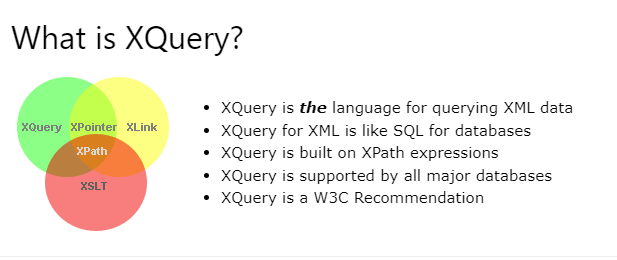
\includegraphics[width=0.75\textwidth,frame]{4221-t8/what.png}
	\caption{Picture cited from W3 School  \url{https://www.w3schools.com/xml/xquery_intro.asp}}
\end{figure}\vspace{-10pt}
\end{frame}

\section*{Section 1 XQuery}

\begin{frame}[fragile]{Question 1.1}
Find the albums where the number of songs is greater than or equal to 3. Return the album title and count sorted by the count with the highest count appearing first. Your query should be written in the form of a FLWOR expression.\\\vspace{10pt}

For reference, your XML output should look somewhat similar to this:\\

\begin{lstlisting}[style=xml-small-nomargin]
<albums>
	<album>
		<title>No War</title>
		<count>4</count>
	</album>
	<album>
		<title>Bua Hati</title>
		<count>3</count>
	</album>
	<album>
		<title>Separuh Jiwaku Pergi</title>
		<count>3</count>
	</album>
</albums>
\end{lstlisting}
\end{frame}

\begin{frame}[fragile]{Question 1.1 Cont.}

\textbf{Solution:}
\begin{lstlisting}[style=xml-small]
<albums>{
	for $album in doc("library.xml")/child::library/child::album
		let $title := $album/child::title/text()
		let $count := count($album/child::songs/child::song)
		where $count ge 3
		order by $count descending
		return
			<album>
				<title>{$title}</title>
				<count>{$count}</count>
			</album>
}</albums>
\end{lstlisting}
\end{frame}

\begin{frame}[fragile]{Question 1.2}
	
Show the title and duration of the songs made by Indonesian artists sorted by duration in descending order. \\\vspace{5pt}
You may find declaring a local helper function as well as the built-in \texttt{tokenize(\$input, \$pattern)} function useful. For reference, your output should look something like this:\\\vspace{5pt}
\begin{columns}
\column{0.5\textwidth}
\begin{lstlisting}[style=xml-small-nomargin]
<songs>
	<song>
		<title>Miliki Diriku</title>
		<duration>10:35</duration>
	</song>
	<song>
		<title>Belajarlah Untuk Cinta</title>
		<duration>10:23</duration>
	</song>
	<song>
		<title>Bua Hati</title>
		<duration>5:35</duration>
	</song>
...
\end{lstlisting}
\column{0.47\textwidth}
\begin{lstlisting}[style=xml-small-nomargin]
...	
	<song>
		<title>Timang-Timang</title>
		<duration>5:13</duration>
	</song>
	<song>
		<title>Separuh Jiwaku Pergi</title>
		<duration>5:00</duration>
	</song>
	<song>
		<title>Hujanpun Menangis</title>
		<duration>4:17</duration>
	</song>
</songs>
\end{lstlisting}
\end{columns}
\end{frame}

\begin{frame}[fragile]{Question 1.2 Cont.}
\textbf{Solution:} Start by declaring a function to get the duration as the number of seconds with type integer:\\\vspace{5pt}
\begin{lstlisting}[style=xml-small]
declare function local:duration-in-sec($duration-str as xs:string) as xs:int {
	let $min-secs := tokenize($duration-str, ':')
	return 60 * xs:int($min-secs[1]) + xs:int($min-secs[2])
};
\end{lstlisting}

Option 1: without \textbf{let}-binding\\\vspace{5pt}
\begin{lstlisting}[style=xml-small]
<songs>{
	for $song in doc("library.xml")/child::library/child::album[child::artists/child::artist/
		child::country = 'Indonesia']/child::songs/child::song
		order by local:duration-in-sec($song/child::duration) descending
		return $song
}</songs>
\end{lstlisting}

\end{frame}

\begin{frame}[fragile]{Question 1.2 Cont.}
Option 2: with \textbf{let}-binding\\\vspace{5pt}
\begin{lstlisting}[style=xml-small]
<songs>{
	for $song in doc("library.xml")/child::library/child::album[child::artists/child::artist/
		child::country = 'Indonesia']/child::songs/child::song
		let $duration := local:duration-in-sec($song/child::duration)
		order by $duration descending
		return $song
}</songs>
\end{lstlisting}

\end{frame}

\begin{frame}[fragile]{Question 1.3}
Show the list of titles of the albums made by Indonesian artists sorted by title. For each album show the songs sorted by duration in descending order.\\\vspace{5pt}
For reference, your HTML output when rendered should look somewhat similar to this: \\\vspace{-5pt}
\begin{figure}
	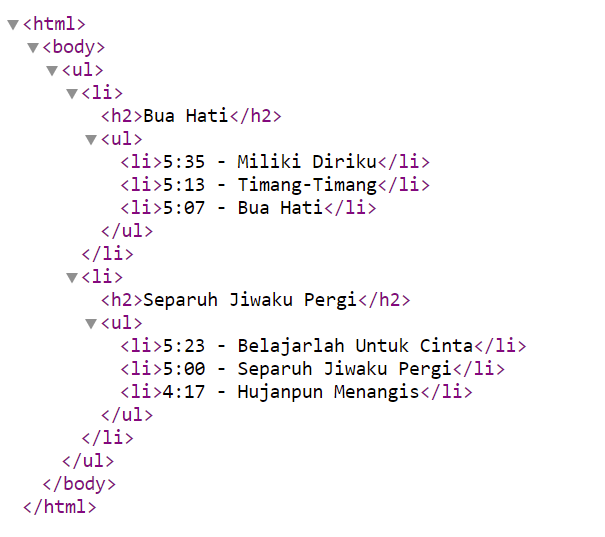
\includegraphics[width=0.5\textwidth,frame]{4221-t8/q3-output.png}
\end{figure}
\end{frame}

\begin{frame}[fragile]{Question 1.3 Cont.}

\textbf{Solution}: \\
\begin{lstlisting}[style=xml-small]
declare function local:duration-in-sec($duration-str as xs:string) as xs:int {
	let $min-secs := tokenize($duration-str, ':')
	return 60 * xs:int($min-secs[1]) + xs:int($min-secs[2])
};
<html>
	<body>
		<ul>{
			for $album in doc("library.xml")/child::library/child::album[child::artists/child::artist/
				child::country = 'Indonesia']
				let $album-title := $album/child::title/text()
				order by $album-title
				return
					<li>
					<h2>{$album-title}</h2>
					<ul>{
						for $song in $album/child::songs/child::song
						order by local:duration-in-sec($song/child::duration) descending
						return
						<li>{$song/child::duration/text()} - {$song/child::title/text()}</li>
					}</ul>
					</li>
		}</ul>
	</body>
</html>
\end{lstlisting}


\end{frame}


\begin{frame}[fragile]{Question 1.4}
Color the songs with a duration greater than or equal to 600 seconds green and otherwise red.\\\vspace{5pt}
Note that ``||'' is used in XQuery for string concatenation. For reference, your HTML output when rendered should look somewhat similar to this: \\\vspace{15pt}
\textbf{Solution shown in the next slide.}
\end{frame}
	
\begin{frame}[fragile]{Question 4 Cont.}

\begin{lstlisting}[style=xml-small-nomargin]
<!-- We keep the function local:duration-in-sec unchanged -->
<html>
	<body>
		<ul>{
			for $album in doc("library.xml")/child::library/child::album[child::artists/child::artist/child::country = 'Indonesia']
				let $album-title := $album/child::title/text()
				order by $album-title
				return
				<li>
				<h2>{$album-title}</h2>
				<ul>{
					for $song in $album/child::songs/child::song
						let $duration := local:duration-in-sec($song/child::duration)
						order by $duration descending
						return
						element li {
							attribute style {
								if ($duration >= 600) then 'color:green;' else 'color:red;'
							},
							$song/child::duration/text() || ' - ' || $song/child::title/text()
						}
				}</ul>
				</li>
		}</ul>
	</body>
</html>
\end{lstlisting}\vspace{5pt}
\end{frame}

\begin{frame}[fragile]{Question 1.5}
Find the albums where the total listening duration (the sum of all the album's songs' duration) is greater than 1100 seconds. The albums should be sorted by title. In the XML output, you should return the album elements that satisfy the constraint with the title and an extra attribute duration. Your main code should be formed as a FLWOR expression. You may use functions you have declared in previous questions.\\\vspace{5pt}
For reference, your XML output should look somewhat similar to this:\\\vspace{5pt}

\begin{lstlisting}[style=xml-small-nomargin]
<albums>
	<album>
		<title>Bua Hati</title>
		<duration>1283</duration>
	</album>
	<album>
		<title>Separuh Jiwaku Pergi</title>
		<duration>1180</duration>
	</album>
</albums>
\end{lstlisting}\vspace{5pt}	
\end{frame}

\begin{frame}[fragile]{Question 1.5 Cont.}
\textbf{Solution}: \\
\begin{lstlisting}[style=xml-small-nomargin]
<!-- We keep the function local:duration-in-sec unchanged -->
<albums>{
	for $album in doc("library.xml")/child::library/child::album
		let $title := $album/child::title/text()
		let $durations := $album/child::songs/child::song/child::duration
		let $total-duration := sum(for $duration in $durations return local:duration-in-sec($duration))
		where $total-duration gt 1100
		order by $title
		return
			<album>
				<title>{$title}</title>
				<duration>{$total-duration}</duration>
			</album>
}</albums>
\end{lstlisting}
\end{frame}


\begin{frame}[fragile]{Question 1.6}
Explain a key difference between the for loop used in XQuery compared to an imperative language such as Python.\\\vspace{10pt}

\textbf{Solution}: \\
XQuery is a functional language. Each iteration is executed in parallel and no communication between the threads are allowed. This is in contrast to imperative languages where the iterations are executed sequentially and may i.e. increment a counter or likewise. See XQuery/FLWOR Expression for more info.

\begin{block}{To read more...}
The XQuery Tutorial on W3 School: \url{https://www.w3schools.com/xml/xquery_intro.asp}
\end{block}	
\end{frame}

\section*{Section 2 XSLT}
\begin{frame}[fragile]{Question (XSL) 2.1}
Write an XSLT stylesheet that displays in a table or a list of an HTML document the name and released year of the albums with genre “Pop” of the XML document.\\\vspace{5pt}
Prefer XSLT template matching with ``\textbf{value-of}'' and ``\textbf{apply-template}'' to imperative control structures (e.g. ``\textbf{for-each}'').\\\vspace{10pt}

\end{frame}

\begin{frame}[fragile]{Question (XSL) 2.1 Cont.}
\textbf{Solution}: (Save the code below into an \textbf{.xsl} file)\\
\begin{lstlisting}[style=xml-small-nomargin]
<?xml version="1.0" encoding="UTF-8"?>
<xsl:stylesheet xmlns:xsl="http://www.w3.org/1999/XSL/Transform" version="1.0">
<xsl:template match="/">
	<html>
		<body>
			<ul>
				<xsl:apply-templates select="child::library/child::album[child::genres/child::genre='Pop']"/>
			</ul>
		</body>
	</html>
</xsl:template>

<xsl:template match="album">
	<li>
		Album <xsl:value-of select="title"/> (<xsl:value-of select="year"/>)
	</li>
</xsl:template>

</xsl:stylesheet>
\end{lstlisting}\vspace{5pt}

\end{frame}

\begin{frame}[fragile]{Question (Transformation) 2.2}
Perform XLST transformation through eXist-db using the XLST file you just created.\\\vspace{5pt}

\textbf{Solution}:

\begin{lstlisting}[style=xml-small-nomargin]
transform:transform(doc("library.xml"), doc("library.xsl"), ())
\end{lstlisting}\vspace{5pt}

\begin{block}{To read more...}
	The XSLT Tutorial on W3 School: \url{https://www.w3schools.com/xml/xsl_intro.asp}
\end{block}	
\end{frame}

\begin{frame}{}
	\centering  
	For any further question, please feel free to email me:\vspace{10pt}
	
	huasong.meng@u.nus.edu \vspace{20pt}
	
	\begin{tcolorbox}
		\begin{center}
			\textcolor{red}{Copyright 2021 Mark H. Meng. All rights reserved.}
		\end{center}
	\end{tcolorbox}
\end{frame}